\documentclass[../../main.tex]{subfiles}

\begin{document}

\clearpage

\section{Matlab}

\begin{fulltheorem}
  Az „M” nyelv jellegzetességei.
\end{fulltheorem}

A \kix{MATLAB} programozási nyelv és egy speciális programrendszer, amelyet
numerikus számítások elvégzésére fejlesztettek ki. A The MathWorks által
kifejlesztett programrendszer képes mátrix számítások elvégzésére, függvények
és adatok ábrázolására, algoritmusok implementációjára és felhasználói
interfészek kialakítására. Habár a szoftver kizárólag numerikus, a MuPAD csomag
hozzáadásával képes matematikai kifejezéseket grafikusan is megjeleníteni.

\subsubsection*{{Semicolon}}
Más programozási nyelvekkel ellentétben, ahol a pontosvessző (\texttt{;})
választja el egymástól a parancsokat, a Matlabban, a parancsok kiírása függ tőle.
Ha egy parancs végén pontosvessző szerepel, akkor nem kerül kiíratásra. Ellenkező
esetben kiíródik. Ha egy parancs vagy függvény nem rendelkezik visszatérési értékkel,
akkor ugyanaz történik a pontosvessző megléte vagy hiánya esetén is.

\subsubsection*{Változók}
\begin{minted}[bgcolor=bg]{matlab}
>> x = 17
x =
 17
>> x = 'hat'
x =
hat
>> x = [3*4, pi/2]
x =
   12.0000    1.5708
>> y = 3*sin(x)
y =
   -1.6097    3.0000
\end{minted}

\subsubsection*{Mátrixok}
\begin{minted}[bgcolor=bg]{matlab}
% Vectors
>> array = 1:2:9
array =
 1 3 5 7 9

>> array = 1:5
array =
 1 2 3 4 5

% Matrices
>> A = [16 3 2 13;
        5 10 11 8;
        9 6 7 12;
        4 15 14 1]
A =
 16  3  2 13
  5 10 11  8
  9  6  7 12
  4 15 14  1

>> A(2,3)
ans =
 11

>> A(2:4,3:4)
ans =
 11 8
 7 12
 14 1

% Unit matrix
>> eye(3,3)
ans =
 1 0 0
 0 1 0
 0 0 1

% Zero matrix
>> zeros(2,3)
ans =
 0 0 0
 0 0 0

% One matrix
>> ones(2,3)
ans =
 1 1 1
 1 1 1
\end{minted}

\subsubsection*{Grafika}
\begin{minted}[bgcolor=bg]{matlab}
% Plot sine of x
x = 0:pi/100:2*pi;
y = sin(x);
plot(x,y)
xlabel('$x$')
ylabel('$\sin x$')

% Plot sinc as mesh
[X,Y] = meshgrid(-10:0.25:10,-10:0.25:10);
f = sinc(sqrt((X/pi).^2+(Y/pi).^2));
mesh(X,Y,f);
axis([-10 10 -10 10 -0.3 1])
xlabel('$x$')
ylabel('$y$')
zlabel('$\mathrm{sinc}(x; y)$')
hidden off

% Plot sinc as meshgrid
[X,Y] = meshgrid(-10:0.25:10,-10:0.25:10);
f = sinc(sqrt((X/pi).^2+(Y/pi).^2));
surf(X,Y,f);
axis([-10 10 -10 10 -0.3 1])
xlabel('$x$')
ylabel('$y$')
zlabel('$\mathrm{sinc}(x; y)$')
hidden off
\end{minted}

\begin{figure}[H]
  \centering
  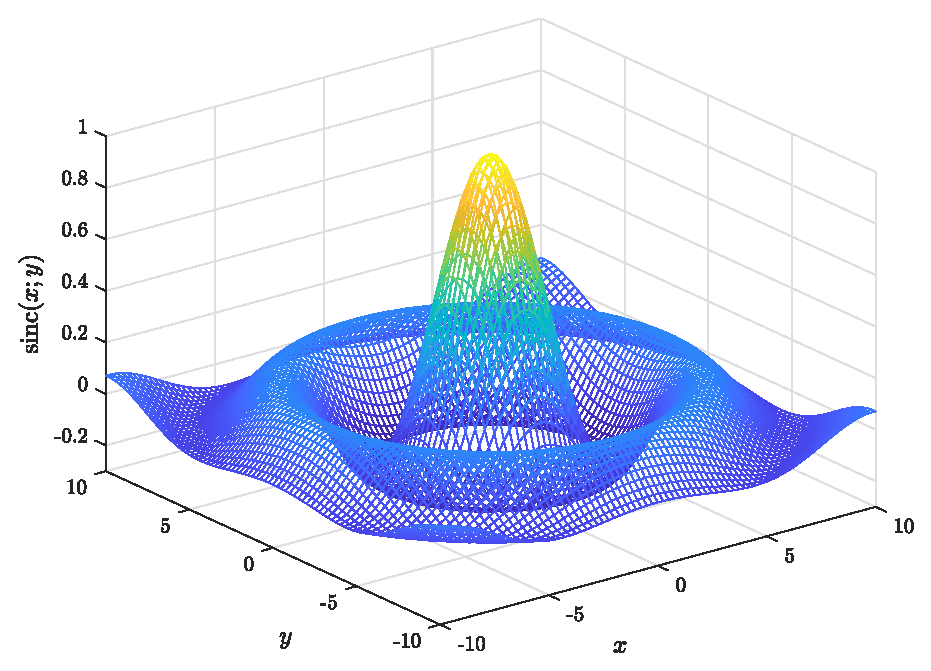
\includegraphics[width=.45\textwidth]{../../static/matlab-ex2}
  \hfill
  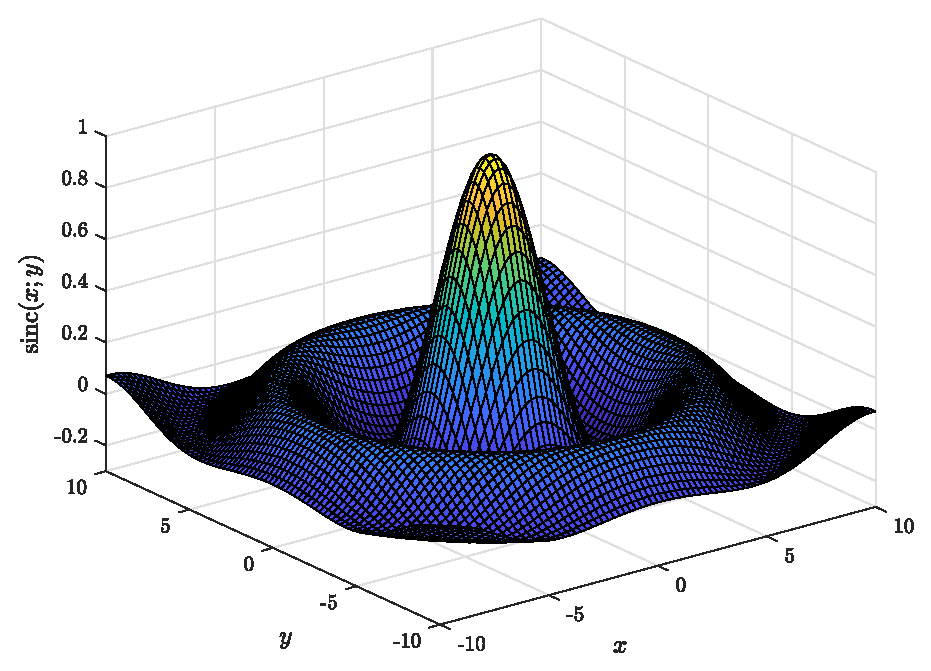
\includegraphics[width=.45\textwidth]{../../static/matlab-ex3}
  \caption{A matlab plotok eredménye}
  \label{fig:matlab}
\end{figure}

\end{document}
